\subsection{The facts, and just the facts}

It is not unusual to make the mistake of trying to keep the user too much information, offering unneccessary or redundant data.\\
 
This defeats the objective of being relevant to the user. We don't want the user to be distracted or lost in the middle
 of a complete but complex data pool that is irrelevant.\\

The objective is not to create specialized users in the field, but to provide them with the
information in a way that they can apply to their daily life and thus improve it. Showing
technical, difficult to interpret data will only deter the user. \\

In complex cases, when dealing with concepts that are not in the users comfort zone, we can resort information
complementary to his disposition so that the user can be informed about the meaning of the data
represented, this practice will provide the user with a greater mastery of the concept and could be more
sure of his reading of the data, since when we direct the user to official sources of information, where they can
get a real explanation, reinforce the credibility of the representations we are making. In any case,
outside of the main representation, because the user will not have to access this information continuously.\\

\subsubsection*{Suggested strategies}

Focus on the objective, show only the data directly related to our goal, do not annotate the data
simply because it appears in the dataset, and don't include distracting technical details irrelevant to the user.

\subsubsection*{In the context of Aire Guru \ldots} 

The dataset used contains data such as the identifier of the measurement station, whether the station is fixed or mobile
and extra-specific measures for an application that is provided by the same company that collects the data. This data is not useful for us.
For our tool, only the coordinates of the measurement station have been used, as well as the time at which the measurement was recorded, and the most relevant value of the five pollutants Co, No2, O3, Pm1, Pm 2.5 and Pm10.\\

In addition, the measurement is unique for everyone and the general, the AQI, the ranges are exactly the same for everyone, so the user just has to make the effort to understand a single concept.\\

If the measure does not exist, we simply ignore it. We do not provide explanations or values such as 0 that can be mis-interpreted, erroneously reading as if there was no pollution.\\


In the following figure we see the difference between the zone history and the personalized, the first of them does not show
the point where the measure was taken since it has been selected in the main map. We also like for the history of
zone there is no filter for hours, since the measurements are reported every hour, this means that we will not find
intermediate measures in the dataset.\\

\newpage
\begin{figure}[ht]
    \centering
    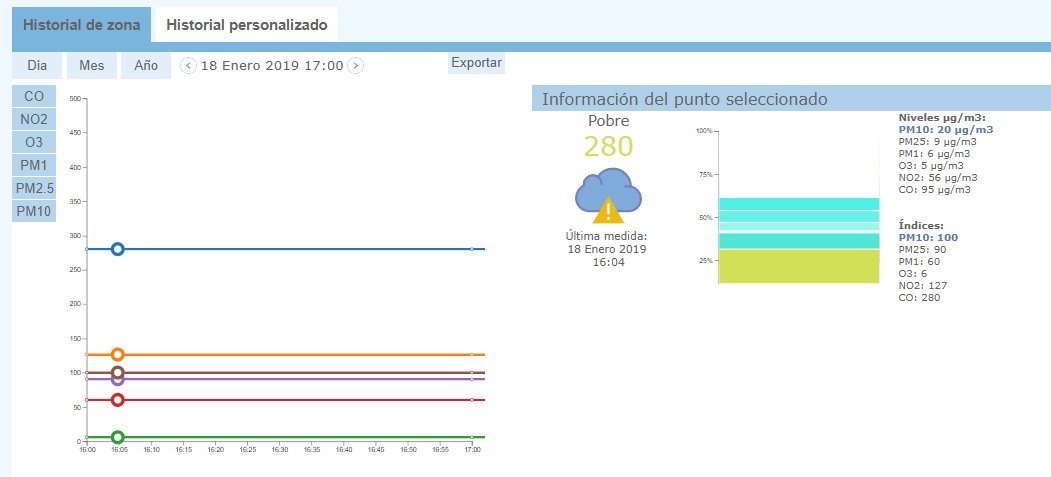
\includegraphics[width=11cm]{zoneRecords}
    \caption{Zone Records}
\end{figure}
\begin{figure}[ht]
    \centering
    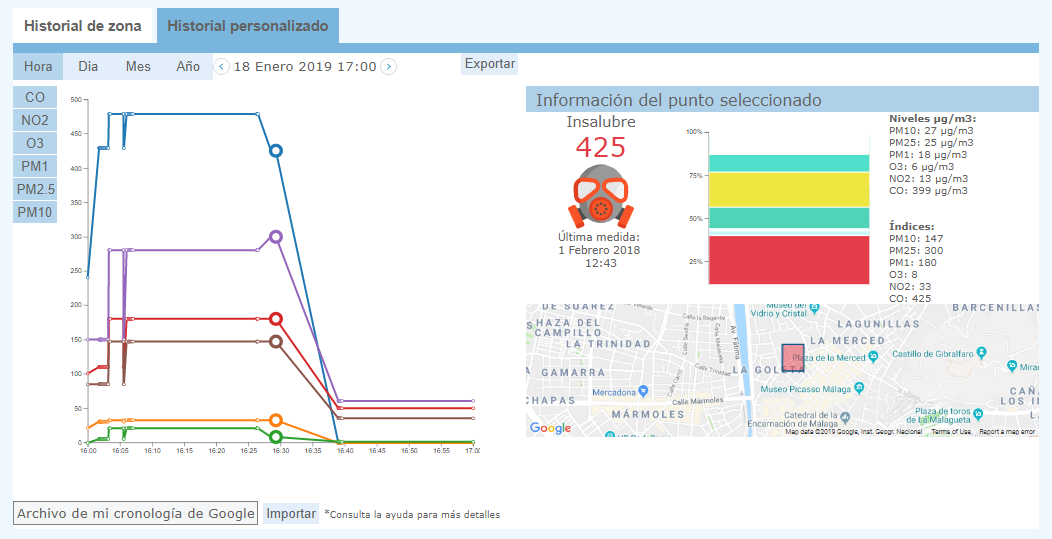
\includegraphics[width=11cm]{personalRecords}
    \caption{Personal Records}
\end{figure}

\subsubsection*{Evaluation}  

\begin{itemize}
    \done The information not relevant to the user has been removed.
    \crossed Exact measurements have been given. This data is quite technical for the user, but 
    it lends veracity to the data. Therefore we have given it a secondary position so it doesn't distract the user.
    \crossed It has implemented a functionality to export the data. The comments of our testers revealed
    that this functionality is not useful for the average user, since they do not have the necessary tools to
    analyze the data and all the information is represented in a better format in the tool itself.
\end{itemize}